% Options for packages loaded elsewhere
\PassOptionsToPackage{unicode}{hyperref}
\PassOptionsToPackage{hyphens}{url}
%
\documentclass[
]{article}
\usepackage{lmodern}
\usepackage{amssymb,amsmath}
\usepackage{ifxetex,ifluatex}
\ifnum 0\ifxetex 1\fi\ifluatex 1\fi=0 % if pdftex
  \usepackage[T1]{fontenc}
  \usepackage[utf8]{inputenc}
  \usepackage{textcomp} % provide euro and other symbols
\else % if luatex or xetex
  \usepackage{unicode-math}
  \defaultfontfeatures{Scale=MatchLowercase}
  \defaultfontfeatures[\rmfamily]{Ligatures=TeX,Scale=1}
\fi
% Use upquote if available, for straight quotes in verbatim environments
\IfFileExists{upquote.sty}{\usepackage{upquote}}{}
\IfFileExists{microtype.sty}{% use microtype if available
  \usepackage[]{microtype}
  \UseMicrotypeSet[protrusion]{basicmath} % disable protrusion for tt fonts
}{}
\makeatletter
\@ifundefined{KOMAClassName}{% if non-KOMA class
  \IfFileExists{parskip.sty}{%
    \usepackage{parskip}
  }{% else
    \setlength{\parindent}{0pt}
    \setlength{\parskip}{6pt plus 2pt minus 1pt}}
}{% if KOMA class
  \KOMAoptions{parskip=half}}
\makeatother
\usepackage{xcolor}
\IfFileExists{xurl.sty}{\usepackage{xurl}}{} % add URL line breaks if available
\IfFileExists{bookmark.sty}{\usepackage{bookmark}}{\usepackage{hyperref}}
\hypersetup{
  pdftitle={Descriptive Analytics},
  pdfauthor={Gabriel Burcea},
  hidelinks,
  pdfcreator={LaTeX via pandoc}}
\urlstyle{same} % disable monospaced font for URLs
\usepackage[margin=1in]{geometry}
\usepackage{longtable,booktabs}
% Correct order of tables after \paragraph or \subparagraph
\usepackage{etoolbox}
\makeatletter
\patchcmd\longtable{\par}{\if@noskipsec\mbox{}\fi\par}{}{}
\makeatother
% Allow footnotes in longtable head/foot
\IfFileExists{footnotehyper.sty}{\usepackage{footnotehyper}}{\usepackage{footnote}}
\makesavenoteenv{longtable}
\usepackage{graphicx,grffile}
\makeatletter
\def\maxwidth{\ifdim\Gin@nat@width>\linewidth\linewidth\else\Gin@nat@width\fi}
\def\maxheight{\ifdim\Gin@nat@height>\textheight\textheight\else\Gin@nat@height\fi}
\makeatother
% Scale images if necessary, so that they will not overflow the page
% margins by default, and it is still possible to overwrite the defaults
% using explicit options in \includegraphics[width, height, ...]{}
\setkeys{Gin}{width=\maxwidth,height=\maxheight,keepaspectratio}
% Set default figure placement to htbp
\makeatletter
\def\fps@figure{htbp}
\makeatother
\setlength{\emergencystretch}{3em} % prevent overfull lines
\providecommand{\tightlist}{%
  \setlength{\itemsep}{0pt}\setlength{\parskip}{0pt}}
\setcounter{secnumdepth}{5}

\title{Descriptive Analytics}
\author{Gabriel Burcea}
\date{09/07/2020}

\begin{document}
\maketitle

{
\setcounter{tocdepth}{2}
\tableofcontents
}
\hypertarget{i.-descriptive-analytics}{%
\subsection{I. Descriptive analytics}\label{i.-descriptive-analytics}}

Exploratory questions of interest are: 1. How does symptom profile map
to mild/moderate/severe? 2. Does symptom profile differ by underlying
co-morbidity?

Answering to first question: 1. How does symptom profile map to
mild/moderate/severe?

We choose to look at the most common symptoms according to UK guidelines
in patients who reported that they had a Covid 19 positive test. We look
at these symptoms according to whether they were reported as
mild/moderate/severe
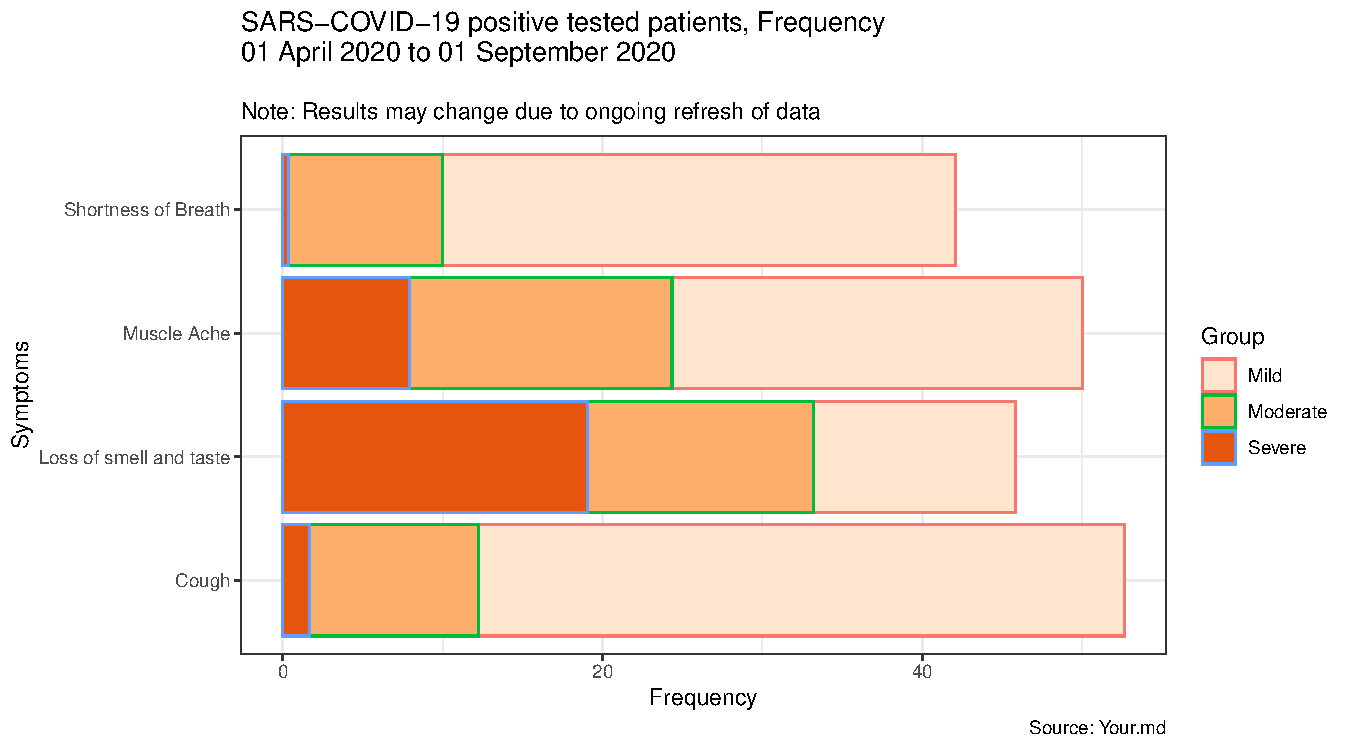
\includegraphics{Final_descript_analysis_files/figure-latex/symptoms_covid_in_resp-1.pdf}
Cough, followed by muscle ache are the most symptoms in patient who
declared they had a Covid-19 positive test. Loss of smell and shorthness
of breath are next. Yet, as observed there are different levels of
severity, were mild form of symptoms are reported.

\begin{longtable}[]{@{}lrrrrrrrr@{}}
\toprule
Group & Count\_cough & Cough & Count\_muscle\_ache & Muscle Ache &
Count\_shortness\_breath & Shortness of Breath &
Count\_loss\_smell\_taste & Loss of smell and taste\tabularnewline
\midrule
\endhead
Mild & 214 & 40.377358 & 136 & 25.660377 & 170 & 32.0754717 & 67 &
12.64151\tabularnewline
Moderate & 56 & 10.566038 & 87 & 16.415094 & 51 & 9.6226415 & 75 &
14.15094\tabularnewline
Severe & 9 & 1.698113 & 42 & 7.924528 & 2 & 0.3773585 & 101 &
19.05660\tabularnewline
\bottomrule
\end{longtable}

The next barchart takes into accound all other symptoms for the purpose
of comparison. However, fatigue seems to have the highest countS,
followed by the most common symptoms of Covid-19.

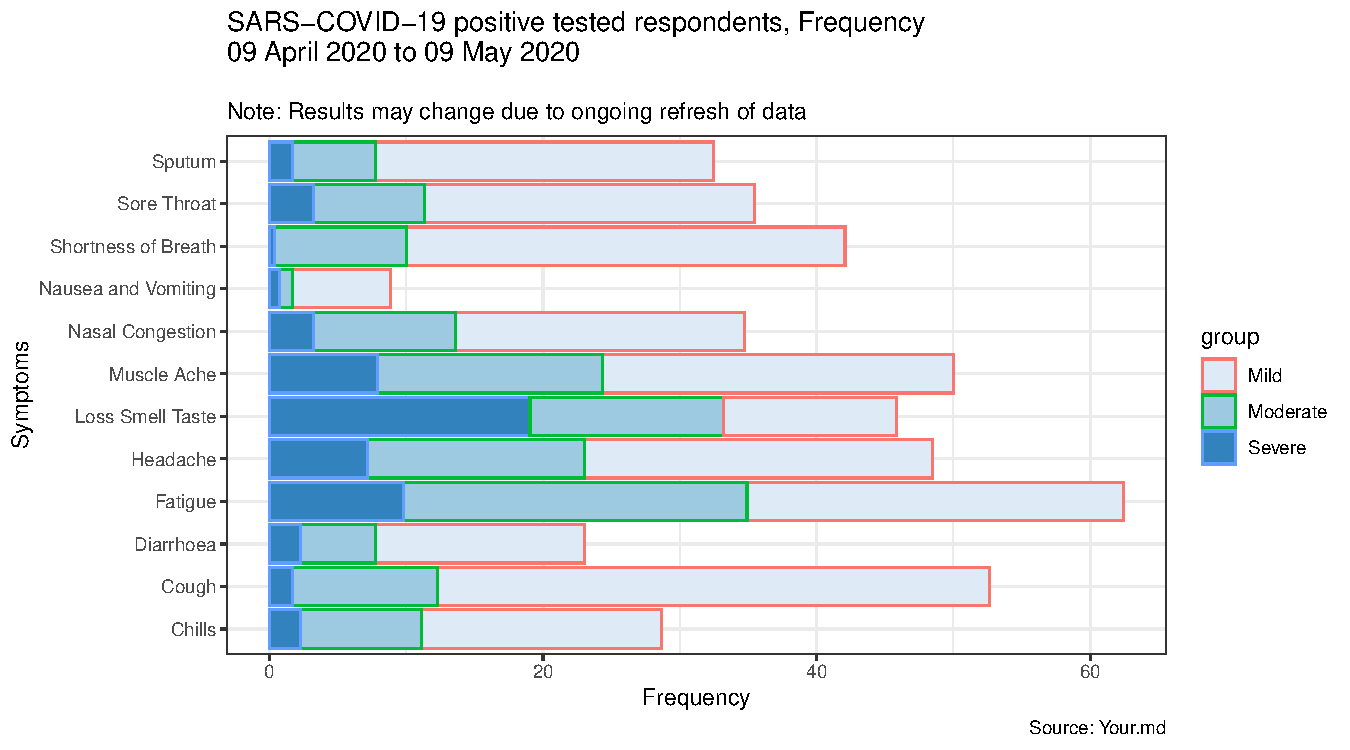
\includegraphics{Final_descript_analysis_files/figure-latex/symptom_profile_all_symptoms-1.pdf}

Table bellow shows the first ten most occurring symptoms taking into
account the level of severity. However, the most common symptoms
expressed in level of severity are Cough as a mild for, shortness of
breath, fatigue, muscle ache and headache, all in a mild form.

\begin{longtable}[]{@{}llrr@{}}
\toprule
group & Event & Count & Frequency\tabularnewline
\midrule
\endhead
Mild & Cough & 214 & 40.37736\tabularnewline
Mild & Shortness of Breath & 170 & 32.07547\tabularnewline
Mild & Fatigue & 146 & 27.54717\tabularnewline
Mild & Muscle Ache & 136 & 25.66038\tabularnewline
Mild & Headache & 135 & 25.47170\tabularnewline
Moderate & Fatigue & 133 & 25.09434\tabularnewline
Mild & Sputum & 131 & 24.71698\tabularnewline
Mild & Sore Throat & 128 & 24.15094\tabularnewline
Mild & Nasal Congestion & 112 & 21.13208\tabularnewline
Severe & Loss Smell Taste & 101 & 19.05660\tabularnewline
\bottomrule
\end{longtable}

\begin{longtable}[]{@{}lrr@{}}
\toprule
Group & Count & Frequency\tabularnewline
\midrule
\endhead
Mild & 17003 & 0.8628774\tabularnewline
Moderate & 2385 & 0.1210353\tabularnewline
Severe & 317 & 0.0160873\tabularnewline
\bottomrule
\end{longtable}

Respondents who tested covid positive have reported the 37.5-38
temperature as the most frequent.

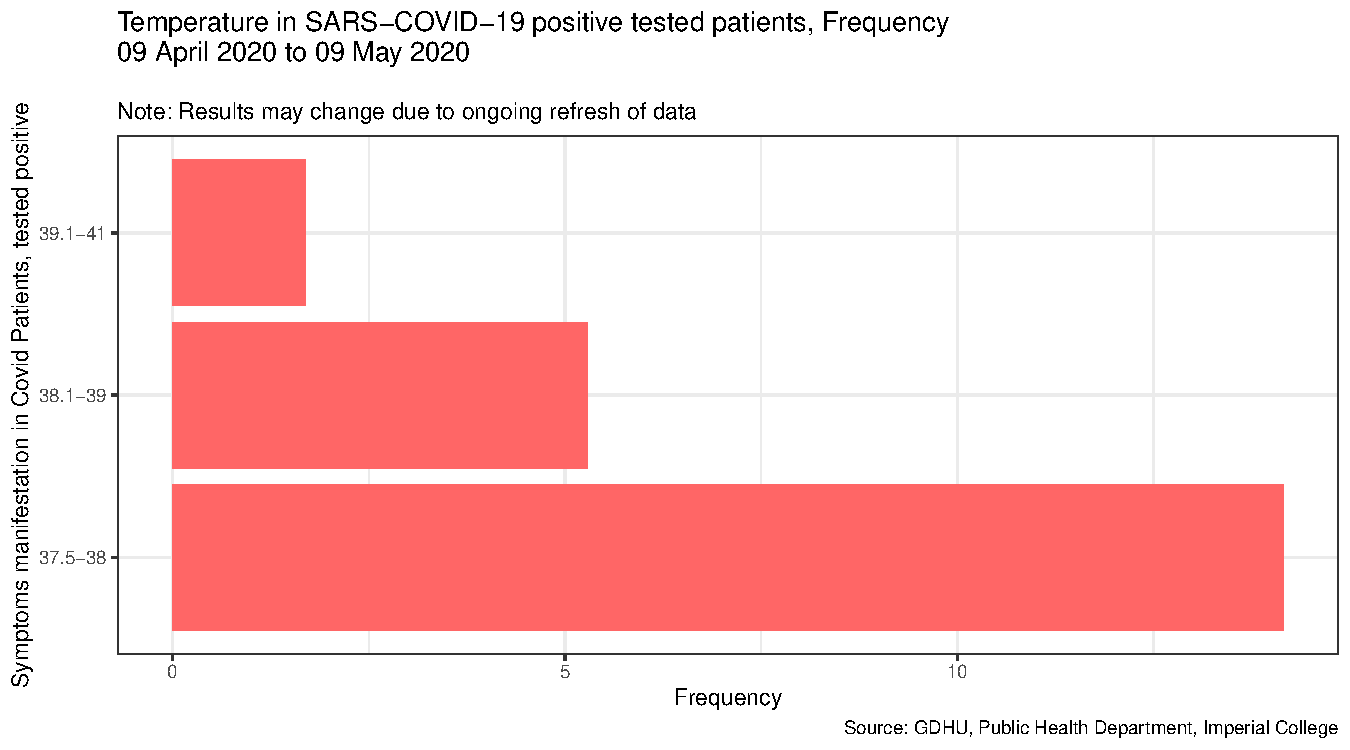
\includegraphics{Final_descript_analysis_files/figure-latex/temperature-1.pdf}

\hypertarget{a-tibble-3-x-3}{%
\section{A tibble: 3 x 3}\label{a-tibble-3-x-3}}

Group Count Frequency 1 37.5-38 75 14.2 2 38.1-39 28 5.28 3 39.1-41 9
1.70

The bellow barchart maps the patients who claimed their symptoms were
overall mild. What symptoms did they have? The most prevalent symptoms
are cough, fatigue, sore throat, sputum and muscle ache.

\hypertarget{htmlwidget-1c4ff5e95f50863b0e26}{}
\begin{plotly}

\end{plotly}

The most prevalent symptoms are cough, fatigue, sore throat, sputum and
muscle ache.

\begin{longtable}[]{@{}llrr@{}}
\toprule
Group & Event & Count & Frequency\tabularnewline
\midrule
\endhead
Mild & Cough & 6971 & 40.99865\tabularnewline
Mild & Fatigue & 6112 & 35.94660\tabularnewline
Mild & Sore Throat & 6057 & 35.62313\tabularnewline
Mild & Sputum & 5400 & 31.75910\tabularnewline
Mild & Muscle Ache & 5254 & 30.90043\tabularnewline
Mild & Headache & 4805 & 28.25972\tabularnewline
Mild & Nasal Congestion & 4184 & 24.60742\tabularnewline
Mild & Shortness of Breath & 4041 & 23.76639\tabularnewline
Mild & Chills & 2217 & 13.03888\tabularnewline
Moderate & Fatigue & 2009 & 11.81556\tabularnewline
\bottomrule
\end{longtable}

Bellow chart is mapping the patients claiming their symptoms were
overall moderate. What symptoms did they have?

\hypertarget{htmlwidget-a0233c8e1c70406533cc}{}
\begin{plotly}

\end{plotly}

Shortness of breath, cough, sputum fatigue as a mild form followed by
moderate fatigue are the first 5 symptoms declared by the respondents of
Your.md app.

\begin{longtable}[]{@{}llrr@{}}
\toprule
Group & Event & Count & Frequency\tabularnewline
\midrule
\endhead
Mild & Shortness of Breath & 953 & 39.95807\tabularnewline
Mild & Cough & 938 & 39.32914\tabularnewline
Mild & Sputum & 791 & 33.16562\tabularnewline
Mild & Fatigue & 746 & 31.27883\tabularnewline
Moderate & Fatigue & 707 & 29.64361\tabularnewline
Mild & Sore Throat & 704 & 29.51782\tabularnewline
Mild & Muscle Ache & 679 & 28.46960\tabularnewline
Mild & Headache & 645 & 27.04403\tabularnewline
Mild & Nasal Congestion & 613 & 25.70231\tabularnewline
Moderate & Muscle Ache & 504 & 21.13208\tabularnewline
\bottomrule
\end{longtable}

Bellow chart is mapping the patients claiming their symptoms were
overall severe, What symptoms did they have?

\hypertarget{htmlwidget-50c159696e76c2e39b52}{}
\begin{plotly}

\end{plotly}

Cough, sputum, sore throat, shortness of breath and headache in mild
form are the first 5 symptoms.

\begin{longtable}[]{@{}llrr@{}}
\toprule
Group & Event & Count & Frequency\tabularnewline
\midrule
\endhead
Mild & Cough & 93 & 29.33754\tabularnewline
Mild & Sputum & 83 & 26.18297\tabularnewline
Mild & Sore Throat & 69 & 21.76656\tabularnewline
Mild & Shortness of Breath & 67 & 21.13565\tabularnewline
Mild & Headache & 66 & 20.82019\tabularnewline
Moderate & Fatigue & 64 & 20.18927\tabularnewline
Mild & Fatigue & 63 & 19.87382\tabularnewline
Mild & Nasal Congestion & 60 & 18.92744\tabularnewline
Moderate & Shortness of Breath & 59 & 18.61199\tabularnewline
Mild & Muscle Ache & 50 & 15.77287\tabularnewline
\bottomrule
\end{longtable}

As a conclusion we may pressume a symptom trajectory in covid-19
positive tested. Mild sore throat which then progresses to a cough, and
shortness of breath?

\begin{enumerate}
\def\labelenumi{\arabic{enumi}.}
\setcounter{enumi}{1}
\tightlist
\item
  Does symptom profile differ by underlying co-morbidity?
\end{enumerate}

The bar chart bellow shows symptom across co-morbidity groups. By
observing the obesity and hypertensive patients, although we see a
similar pattern in symptom manifestation, there are slight differences
when it comes to sputum and sore throat. In hypertensive respondents
sore throat is more prominent than in obese respondents, which are
experiencing more sputum. This is not the same with respondent with
asthma, which are experiencing sputum and shortness of breath, where
sore throat comes on the fourth place, after muscle ache.

\hypertarget{htmlwidget-b4c367d754945f74ab3a}{}
\begin{plotly}

\end{plotly}

\hypertarget{a-tibble-324-x-4}{%
\section{A tibble: 324 x 4}\label{a-tibble-324-x-4}}

\hypertarget{groups-morbidity-9}{%
\section{Groups: Morbidity {[}9{]}}\label{groups-morbidity-9}}

Morbidity Count Percentage Symptom\\
~\\
1 High Blood Pressure (hypertension) 1812 10.9 Cough\\
2 High Blood Pressure (hypertension) 1666 10.1 Sore Throat 3 High Blood
Pressure (hypertension) 1631 9.85 Sputum\\
4 Obesity 1570 10.5 Cough\\
5 High Blood Pressure (hypertension) 1547 9.34 Fatigue\\
6 Obesity 1422 9.49 Sputum\\
7 High Blood Pressure (hypertension) 1406 8.49 Muscle Ache 8 Obesity
1398 9.33 Sore Throat 9 Obesity 1397 9.33 Fatigue\\
10 Obesity 1310 8.75 Muscle Ache \# \ldots{} with 314 more rows

\hypertarget{htmlwidget-38330dde85c705e7f02b}{}
\begin{plotly}

\end{plotly}

\hypertarget{htmlwidget-0cb2c06cc2dabc5d95a8}{}
\begin{plotly}

\end{plotly}

\hypertarget{htmlwidget-add28e73bbe5733dc9a8}{}
\begin{plotly}

\end{plotly}

\hypertarget{htmlwidget-50bba5cef10f8a842f58}{}
\begin{plotly}

\end{plotly}

Overview of groups of respondents with symptoms and tested positive.

Looking at respondents who are covid positive and the symptoms.

\hypertarget{htmlwidget-9fcbbf8f0ede2e0976be}{}
\begin{plotly}

\end{plotly}

Looking at respondents who declared no covid - this is visualised in
order to decide whether this group shall be added to the analysis as
forming the group 0.

\hypertarget{htmlwidget-31950989922c4f93d372}{}
\begin{plotly}

\end{plotly}

\hypertarget{htmlwidget-600a3309a17c017e67a5}{}
\begin{plotly}

\end{plotly}

\end{document}
